% !TeX root = ../tfm.tex
%! TEX root = ../tfm.tex

En este capítulo expondremos las tareas realizadas para obtener una base de datos propia para el posterior entrenamiento del sistema, así como la descripción de la misma y de los estudios previos de las tramas obtenidas que nos ayudarán en el capítulo siguiente a la definición del modelo y parámetros del algoritmo.

Como ya hemos presentado anteriormente en la sección \ref{sec:req:bases:datos}, nos encontramos ante la falta de una base de datos para entrenar el modelo del producto final. Al tratarse de un modelo experimental es necesario conseguir un conjunto de datos lo más parecido posible a los capturados por la plataforma física utilizada. A su vez es necesario validar la capacidad de esta plataforma para servir al propósito de este trabajo. Así, con esta doble tarea de generar una bases de datos y confirmar que la plataforma cubre nuestras necesidades funcionales realizamos el primer desarrollo propio del trabajo.

\section{Elección y definición de la plataforma}\label{sec:imp:plataforma}

Tras el análisis de requisitos se concreta la plataforma de servicios en la nube, dispositivo y entorno de desarrollo y pruebas a utilizar.

\paragraph{Plataforma de red}\\
Para el servidor optamos por una arquitectura de microservicios usando la plataforma de AWS Lambda con almacenamiento en S3. Como ya se ha expuesto en el análisis de requisitos, esta plataforma integra todas las funciones requeridas y permite su programación en \textit{JavaScript}, lenguaje con el que el autor está familiarizado. Además, dispone de una interfaz de programación pública que permitirá facilitar la generación y entrenamiento de modelos al poder interconectar programáticamente los sistemas usados para el entrono de entrenamiento y validación de modelos con la plataforma de implementación.

\paragraph{Dispositivo de captura y procesado}\\
Para el dispositivo móvil usamos un reloj inteligente Fossil Sport Gen. 3 con sistema operativo WearOS y por tanto compatible con el ecosistema Android. El formato de reloj de pulsera es fácilmente reconocible y familiar para el grupo de usuarios objetivo (que recordemos, está formado mayoritariamente por personas de edad avanzada). El único mantenimiento a realizar de forma periódica es el de realizar un proceso de carga periódico y no dista mucho del mantenimiento de los relojes mecánicos con resortes para acumular energía potencial. Así, el hecho de remontuar, el popular \textit{dar cuerda}, un reloj mecánico es muy similar al proceso de carga. Incluso los intervalos son equiparables, ya que en el caso del dispositivo elegido se puede realizar cada dos días, y se completa en menos de una hora.

Esta plataforma cumple con las exigencias funcionales ya que permite desarrollar aplicaciones y portar modelos de redes de neuronas usando \tflite/. Al contar con 512MBytes de memoria RAM, nos permitirá cargar modelos de tamaño pequeño o medio, aunque sea probablemente el procesador quien limite el tamaño del modelo debido a su baja capacidad de cálculo al disponer de una GPU muy limitada, si bien es uno de los microprocesadores más potentes que pueden encontrarse en el mercado de dispositivos llevables sin reducir en exceso la autonomía, como ya hemos visto. El dispositivo además se ofrece a un precio competitivo (cercano a los 100€) que sin ser un requisito si es un punto a tener en cuenta. Mas información sobre el mismo, características técnicas y sensores se encuentran listadas en el \autoref{app:plataforma}.

\paragraph{Entorno de desarrollo}\\
El la generación, entrenamiento, análisis y evaluación de modelos se realiza usando Keras/Tensorflow corriendo en la plataforma Google Colab (\url{https://research.google/}). Este entorno permite generar y trabajar con modelos \tensorflow/ \tflite/ y al basarse en Python 3.x es fácil integrar la generación de modelos con el sistema de servidor en la nube de AWS (con librerías como \textit{boto3} (\url{https://github.com/boto/boto3}). En concreto el sistema guardará todos los modelos generados, historial del entrenamiento, gráficas y resultados varios en el servidor, y recuperará los datos de entrenamiento (tanto las sesiones obtenidas con \accelcapture/ como \sisfall/) del mismo de forma dinámica. Colab permite ejecutar el código en potentes servidores multiprocesador con unidades GPU y/o TPU. En la \autoref{app:colab} se encuentran listados con información de los servidores.


\section{Captura de datos: \accelcapture/}\label{sec:imp:accelcapture}

Bautizamos como \accelcapture/ al sistema de adquisición de tramas o secuencias de la aceleración registrada por el sensor situado en un reloj inteligente son sistema operativo WearOS. La aplicación está diseñada para una vez activada, ejecutarse en segundo plano, detectando actividad, guardando las medidas del acelerómetro y enviando estas secuencias de medidas al un servidor por Internet.

Con esta aplicación el objetivo es doble: probar las capacidades del sistema para albergar la futura implementación del sistema de detección de caídas y obtener un conjunto suficiente de datos para realizar el entrenamiento del modelo de detección de caídas que se usará en el sistema. Dado que la arquitectura de \accelcapture/ como de la futura \ifell/ (la aplicación de detección de caídas en si) comparten gran similitud en su estructura o arquitectura y comparten algunos módulos o clases.

El código de las funciones lambda AWS puede consultarse el el \autoref{app:codigo} mientras que el de la aplicación\accelcapture/ está disponible para descarga en \url{https://github.com/aberaza/accelCapture}.

\subsection{Funcionamiento de la aplicación}\label{sub:accelcapture:flujo}

La función principal de \accelcapture/ es la de permanecer como un servicio en segundo plano encargado de la lectura de los datos del acelerómetro del sistema. Las única interacción necesaria por parte del usuario es la de activar el servicio de captura una primera vez desde la interfaz de usuario que ofrece la aplicación tal y como se muestra en la \autoref{sub:accelcapture:interfaz}. Una vez realizado este paso, y la etapa opcional de introducir el nombre del usuario, el programa funciona de manera persistente en un segundo plano, capturando datos y enviándolos a un servidor en Internet para su tratamiento.

En cuanto al funcionamiento del servicio, se describe en el diagrama \ref{fig:capturaFlow}. La aplicación, una vez en ejecución tiene dos estados posibles: \textit{Reposo} y \textit{Grabando}. Cuando se encuentra en \textit{Reposo} la aplicación lee muestras en busca de actividad y en caso de detectar actividad, pasaría al siguiente estado: \textit{Grabando} en el cual almacena las muestras leidas para enviarlas al servidor cuando deje de medir actividad y vuelva a cambiar de estado.

\figura[0.70]{capturaFlujo}{fig:capturaFlow}{Flujo de trabajo de la aplicación \accelcapture/}

Si entramos en más detalle, el sistema lee muestras de la aceleración capturadas por un sensor triaxial, por lo que obtenemos las componentes en los tres ejes. Aunque almacenamos las componentes de forma individual en cada muestra, para el algoritmo de la aplicación trabajaremos con la norma o módulo del vector aceleración que denotaremos como $\|\vec{A}\|$ para no confundir con el valor absoluto. Dicho esto, el sistema mantiene en todo momento una ventana con los últimos 5 segundos de actividad. Con cada nueva muestra calcula dos índices para detectar actividad o la ausencia de esta, y cambiar en consecuencia de un estado a otro.

El índice de actividad usado es la variación de aceleración entre dos muestras consecutivas $\Delta \|\vec{A}_i\|$ tal y como define la fórmula:
\[
  \Delta \|\vec{A}_{i}\|=\left\{
    \begin{array}{lcl}
      |\|\vec{A}_i\| - g|       & si & i = 0 \\
      |\|\vec{A}_i\| - \|\vec{A}_{i-1}\|| & si & i > 0 \\
    \end{array}
    \right.
\]\\

Donde:\\
$g$ corresponde a la aceleración de la gravedad terrestre o 9,8\ms2/\\
$\|\vec{A}_n\|$ es la norma o módulo del vector aceleración en el instante $n$ .

Este índice se usa para los dos mecanismos de detección de actividad de la aplicación:

\begin{enumerate}
  \item \textbf{Movimiento repentino} Se activa si en cualquier instante el valor leida es mayor de $\Delta \|\vec{A}_i\|\geq2g$. Solo permite detectar actividad.
  \item \textbf{Movimiento prolongado} Es un comparador con histéresis. Activado cuando la aceleración promedio del contenido del buffer es superior a $\frac{1}{250}\sum_{t-250}^t\|\vec{A}_i\|\geq0,3m/s^2$. Se desactiva cuando la misma medida baja del umbral $\frac{1}{250}\sum_{t-250}^t\|\vec{A}_i\|<0,25m/s^2$.
\end{enumerate}

La cota de detección de movimiento repentino se calcula a partir de los resultados obtenidos por \citeA{Bourke2006} para la medición de la cintura por ser la que menor aceleración registra. La diferencia entre la aceleración de pico y de valle usada por bourke es de $\Delta A = (2,74 - 0,60)g = 2,14g$ redondeando a la baja a 2\g/ para garantizar la detección de todos los eventos de este tipo. Finalmente, la cota del detector de actividad prolongada, fijada en 0,3\ms2/, se mide de forma experimental resultado de promediar el vector para realizar el movimiento de leer la hora en el reloj (\autoref{fig:accelMirarReloj}) y volver a la posición de reposo durante la ventana de 5 segundos que usa la aplicación. En caso de activarse alguno de estos mecanismos, el servicio considera que ha detectado una actividad y cambia al estado \textit{Grabando}. En este estado, se recuperan los 5 segundos ya almacenados en el buffer de detección de actividad (se recuperan las tres componentes de la aceleración, no el índice de actividad) y se añaden nuevas muestras sin límite de duración hasta que se vuelva al estado \textit{Reposo} por ausencia de actividad. En esta última transición se enviarán las muestas capturadas con información adicional al servidor tal y como se define en la \autoref{sub:accelcapture:red}.

Finalmente, para volver al estado de \textit{Reposo} el único mecanismo que lo permite es el comparador de movimiento prolongado si durante 5 segundos el promedio del índice de actividad es inferior a 0,25. Esta cifra se elige para evitar la proliferación de capturas de sesiones de muy corta duración convirtiendo el sistema en un comparador con histéresis.

\figura[0.5]{MirarRelojAccel}{fig:accelMirarReloj}{$|A|$ y $\Delta A$ resultantes de mirar el reloj}

\subsection{Interfaz de Usuario}\label{sub:accelcapture:interfaz}

La interfaz de usuario de la aplicación permite gestionar y observar el estado del servicio de captura así como definir el identificador de usuario al que pertenece la sesión. Como puede observarse en las capturas de pantalla de la \autoref{fig:accelcapture:UI} se muestra en la parte inferior de la pantalla un boton con información del estado actual del servicio. El botón al ser pulsado alterna entre los estados \textit{activado} y \textit{desactivado}. En la parte superior de la pantalla se muestra la información del identificador de usuario o \textit{nombre} al que se asociarán todas las sesiones registradas. Este identificador puede modificarse desde el mismo reloj. Una vez activado el servicio de captura, puede esconderse interfaz y volver al modo reloj ya que el servicio sigue trabajando de fondo.
\begin{figure}[htb!]
  \centering
  \begin{subfigure}[b]{0.30\textwidth}
      \centering
      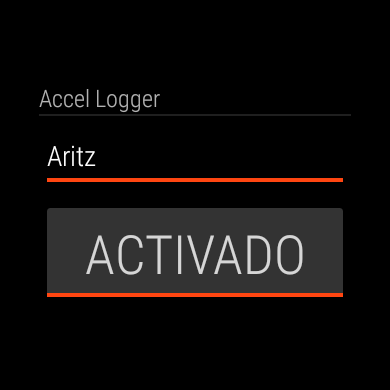
\includegraphics[width=\textwidth]{accelCaptureAct.png}
      \caption{\accelcapture/ Activado}
      \label{fig:accelCapture:UI1}
  \end{subfigure}
  \hfill
  \begin{subfigure}[b]{0.30\textwidth}
      \centering
      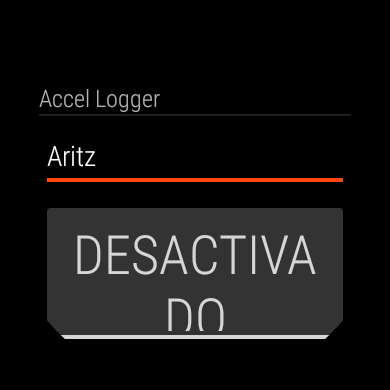
\includegraphics[width=\linewidth]{accelCaptureDes.png}
      \caption{\accelcapture/ Desactivado}
      \label{fig:accelCapture:UI2}
  \end{subfigure}
  \hfill
  \caption{\label{fig:accelcapture:UI} Interfaz de usuario de \accelcapture/}
\end{figure}


\subsection{Arquitectura}\label{sub:accelcapture:archi}


Desde el punto de vista del sistema consta de dos componentes: una unidad de adquisición de datos, el propio reloj, y una segunda unidad de almacenamiento situada en la nube. La estructura de la aplicación se compone de tres bloques funcionales principales tal y como puede apreciarse en el diagrama de clases de la \autoref{fig:accelcaptureClasesUml}.

\figura[0.47]{accelcaptureClassUML}{fig:accelcaptureClasesUml}{Diagrama de clases de \accelcapture/}


\paragraph{MainWearActivity}\\
Es el punto de entrada de la aplicación. Genera la interfaz gráfica y permite introducir el nombre el usuario a la vez que verificar el estado del servicio de captura de datos e iniciar o parar su ejecución.

\paragraph{SensorsReader}\\
El nucleo principal de la plicación. Un servicio que al ser creado se registra para recibir eventos y lecturas del sensor de aceleración triaxial del reloj. Posee una cola circular donde almacena los últimos 5 segundos de muestras (si por ejemplo la velocidad de lectura del sensor es de $1/50$, el buffer posseerá $50 * 5 = 250$ muestras).
Es este servicio el que implementa la lógica descrita en el Apartado~\ref{sub:accelcapture:flujo} tal y como se observa en la \autoref{fig:capturaFlow}, leyendo procesando y almacenando los datos del sensor de aceleración. Tras cada muestra el algoritmo evalúa la variación de la aceleración usando para ello el tercer bloque funcional \textit{ActivityRecognition}. Este bloque es a su vez el encargado de enviar la información de las sesiones capturadas al servidor vía Internet.

\paragraph{ActivityRecognition}\\
Este bloque lo componen los algoritmos de detección de actividad explicados anteriormente. Este módulo propone una interfaz común para poder registrarse y recibir información del módulo \textit{SensorReader} y enviar a su vez eventos que pueda interpretar como son la detección o no de actividad.


\subsection{Envío y Formato de los datos}\label{sub:accelcapture:red}

El objetivo último de \accelcapture/ es el de obtener y almacenar estas tramas o sesiones de actividad para su posterior tratamiento. Este paso se realiza enviando las información a un servidor. Mediante las múltiples capacidades de conexión que tiene el dispositivo (Wifi y Bluetooth + Móvil) que le permiten conectarse desde prácticamente cualquier ubicación y enviar y recibir información. Esta autonomía de funcionamiento permite validar en primera instancia el requisito de no necesitar de infraestructura para el funcionamiento de la aplicación final. Al haber logrado una plataforma autónoma con \accelcapture/, que requiere de una conexión con un servidor, lograrlo con \textit{iFell}, que no tiene necesidad de conexión alguna, debería ser trivial. Esta capacidad de conexión permite poder obtener datos de usuarios de forma remota sin necesidad de ninguna manipulación para obtenerlos una vez usen la aplicación.

Tal y como se menciona en el \apartado{sec:req:nube}, la plataforma en la nube se implementa usando los servicios de AWS. Para esta función crea un microservicio que expone públicamente una \textit{API}(lista de funciones de acceso público que ofrece una biblioteca de programación) del tipo \textit{REST}(Arquitectura que implementa una interfaz sobre el protocolo \textit{HTTP}). Este servicio, definido en la \autoref{tab:accelcapture:api} se encargará de recibir la llamadas de la aplicación y guardar el contenido en un archivo \textit{JSON} (lenguaje de definición de estructuras de datos que usa la notación de JavaScript).

\tablas{tab:accelcapture:api}{API del servidor \accelcapture/}{llll}{
  Método  & URL         & Carga         & Función lambda    \\ \midrule
  POST    & /saveAccel  & AccelSession  & saveToS3()  \\
}{2}

La estructura almacenada se muestra en la \autoref{tab:accelcapture:accel_session} la denominamos \textit{AccelSession}. Este objeto contiene información sobre el sensor (error y frequencia de muestreo), fecha de la captura así como unos identificadores del usuario y de la sesión además de la información capturada en los tres ejes del acelerómetro.



\begin{table}[!htbp]
  \centering
  \subtabla[1.0]{tab:accelcapture:accel_session}{Descripción del Objeto AccelSession}{lll}{
Campo           & Tipo Dato     & Descripción \\ \hline
\textit{uid}    & Alfanumérico  & Identificador único de usuario \\
\textit{sid}    & Alfanumérico  & Identificador único de sesión \\
\textit{sensorResolution} & Real & Resolución del sensor (en \ms2/) \\
\textit{sensorMaxRange} & Real  & Valor máximo de la medida (en \ms2/) \\
\textit{startTime} & Entero     & Tiempo EPOCH del inicio de la sesión (en segundos) \\
\textit{samples}  & Entero      & Número de muestras de la sesión \\
\textit{triggerMethod} & Texto  & Nombre del evento que inició la sesión de captura \\
\textit{sessionData} & SessionData & Estructura con los datos capturados del sensor \\
}{}{2}

%\hspace{\fill}
\subtabla[1.0]{tab:accelcapture:session_data}{Descripción del Objeto SessionData}{lll}{
Campo           & Tipo Dato     & Descripción \\ \hline
\textit{duration} & Entero      & Duración, en $\mu s$, de la sesión \\
\textit{activity} & Texto       & Nombre de la actividad realizada durante la captura \\
\textit{rate}   & Entero        & Ratio de muestreo (en $Hz$) \\
\textit{accelerationX} & Lista<Reales> & Lista de valores de la aceleración capturados en el eje X (en \ms2/) \\
\textit{accelerationY} & Lista<Reales> & Lista de valores de la aceleración capturados en el eje Y (en \ms2/) \\
\textit{accelerationZ} & Lista<Reales> & Lista de valores de la aceleración capturados en el eje Z (en \ms2/) \\
}{right}{2}

\caption{\label{tab:accelcapture:data_types} Estructuras de datos de \accelcapture/}
\end{table}


\section{Generación de la base de datos}

Las capturas de actividad se realizan durante un periodo de 6 meses usando la aplicación \accelcapture/ con diversos sujetos. Estas sesiones se realizan llevando el sensor activado 24 horas al día, incluidos los periodos de reposo y sueño, eliminando, de ser necesario, aquellas capturas en las que hubo alguna caida, aunque no se reportó ninguna. El objetivo es capturar la mayor cantidad posible de sesiones de actividades diarias ordinarias, así como otros eventos que, a pesar de que el usuario se encuentre estacionario y en reposo, generan una señal de aceleración no constante como puede ser el uso de diferentes modos de transporte (tren, avión, coche, moto). En total se han registrado más de 100 horas de actividad repartidas en 300 sesiones diferentes.

\subsection{Procesado de las tramas}

A la hora de construir la base de datos, se usarán las estructuras de información almacenadas en el servidor S3. A partir de ellos se construye una matriz o estructura de datos que aúna la información de todas las sesiones. No se realiza ningún filtrado, subsampleado o tratamiento de los datos de aceleración.

\subsubsection{Descripción de la base de datos}

La base de datos final consta de 37563 segundos de actividad capturada en 274 sesiones diferentes realizadas por 3 sujetos de edades que varían entre los 34 y 77 años. Los usuarios han realizado sus activiades diarias con el dispositivo de captura situado en la muñeca izquierda (sin especificar si en la parte superior o inferior de la misma). Los tres sujetos son diestros.

\tabla[0.95\linewidth]{tab:dataset:descripcion}{Resumen de características de la base de datos}{lrl}{
  \textit{Atributo}      & \textit{Valor}   & \textit{Notas} \\\midrule
  Sesiones      & 274     &   \\
  Sujetos       & 3       & Edades: 34, 40 y 77 años \\
  Sensor        & Acel. 3 ejes & Las componentes X, Y, Z\newline se presentan por separado \\
  Frecuencia Muestreo & 50\hz/ & \\
  Unidades medida & \ms2/ & \\
  Resolución del Sensor & 0,0011\ms2/ &  \\
  Valor Máximo & 60\ms2/ & \\
}{2}

\tablan[0.95\linewidth]{tab:dataset:datos}{Referencia de columnas de la base de datos}{llcl}{
  \textit{Columna} & \textit{Tipo} & \textit{Unidades}  & \textit{Descripción} \\ \midrule
  uid             & texto  &        & Identificador único de la sesión \\
  activity        & texto  &        & Nombre de la actividad detectada por la API Google DetectedActivity\tnote{1} \\
  samplerate      & número & \hz/   & Frecuencia de lectura del sensor \\
  trigger         & texto  &        & Nombre del mecanismo de activación que inició la captura \\
  resolution      & número & \ms2/  & Resolución del sensor tal y como informa el SO\\
  max             & número & \ms2/  & Máximo valor para cada muestra tal y como informa el SO\\
  data            & matriz & \ms2/  & arreglos con las lecturas del sensor para las componentes de la aceleración \\
}{
\item [1] \url{https://developers.google.com/android/reference/com/google/android/gms/location/DetectedActivity\#constants}
}{2}





\subsection{Análisis de las tramas}

Con el fin de entender las características de la señal capturada procedemos a analizar, para las componentes X, Y y Z, así como para el módulo del vector aceleración:
\begin{itemize}
  \item La señal temporal de la aceleración $\|\vec{A}_i\|$ y la señal diferencia $\Delta\|\vec{A}_i\|$
    (Figura \ref{fig:dataset:samples})
  \item El comportamiento frecuencial mediante la transformada de Fourier (Figura \ref{fig:dataset:fftsample})
  \item Autocorrelación de la señal temporal y señal diferencia (Figura \ref{fig:dataset:autocorrsample})
\end{itemize}


\begin{figure}[htb!]
  \centering
  \begin{subfigure}[b]{0.48\textwidth}
      \centering
      \pincludegraphics[1.1]{DatasetXYZModSample}
      \caption{Muestra de la componentes X, Y, Z y $|\vec{A}|$}
      \label{fig:dataset:xyzmodsample}
  \end{subfigure}
  \hfill
  \begin{subfigure}[b]{0.48\textwidth}
      \centering
      \pincludegraphics[1.1]{DatasetAutocorrSample}
      \caption{Autocorrelación de las componentes}
      \label{fig:dataset:autocorrsample}
  \end{subfigure}
  \begin{subfigure}[b]{0.48\textwidth}
    \centering
    \pincludegraphics[1.1]{XYZModFFT}
    \caption{Análisis en frecuencia de X, Y, Z y $\|\vec{A}\|$}
    \label{fig:dataset:fftsample}
  \end{subfigure}
  \hfill
  \begin{subfigure}[b]{0.48\textwidth}
    \centering
    \pincludegraphics[1.1]{DatasetAccelSample}
    \caption{Comparación de $\Delta\|\vec{A}\|$ con $\|\vec{A}\|$}
    \label{fig:dataset:accelsample}
  \end{subfigure}
  \caption{\label{fig:dataset:samples} Análisis de una de las muestras capturadas}
\end{figure}

El objetivo de este análisis es encontrar comportamientos cíclicos en la señal que permitan determinar el tamaño del enventanado a utilizar. Los resultados obtenidos muestran que la autocorrelación de la señal es muy baja y por tanto no existen comportamientos cíclicos que justifiquen el uso de ventanas de gran duración. Analizando las secuencias completas los resultados tanto del análisis espectral como de la autocorrelación indican que la señal es prácticamente aleatoria, sin ningún tipo de correlación interna. Con el fin de verificar este resultado, repetimos el estudio (figura \ref{fig:dataset:sub:autocor} )pero esta vez enventandando con 150 muestras, o 3 segundos, la señal.

\begin{figure}[htb!]
  \centering
  \begin{subfigure}[b]{0.48\textwidth}
      \centering
      \pincludegraphics[1.1]{SubseriesAutocorLow}
      \caption{Autocorrelación de una muestra enventanada con actividad}
      \label{fig:dataset:sub:autocorlow}
  \end{subfigure}
  \hfill
  \begin{subfigure}[b]{0.48\textwidth}
      \centering
      \pincludegraphics[1.1]{SubseriesAutocor}
      \caption{Autocorrelación de una muestra enventanada en reposo}
      \label{fig:dataset:sub:autocorhigh}
  \end{subfigure}
  \caption{\label{fig:dataset:sub:autocor} Estudio de la autocorrelación de la señal enventanada}

\end{figure}

Los resultados se repiten en su mayoría, la señal no presenta periodicidades a destacar salvo cuando se analizan muestras en reposo. En estas suele apreciarse un tono de baja frecuencia (entre 4 y 12\hz/) que atribuimos a un harmónico del pulso en reposo del sujeto que se introduce por efecto del filtrado digital a 50\hz/ que realiza el dispositivo de captura. Al no haber encontrado ninguna componente espectral predominante o ninguna tendencia temporal, tomaremos como tamaño de ventana el doble del periodo que contiene una caída. La estimación de la duración de una caída varía según el estudio, pero tomaremos el acercamiento de que la caída ocurre en la ventana de dos segundos centrada en el instante de máxima aceleración \cite{Sucerquia2017}. 

\subsubsection{Equiparación con \sisfall/}

El siguiente ejercicio a realizar es comparar ciertos parámetros con los de la base de datos \ifell/.  A pesar de que ésta última no se capturó desde desde la misma posición, dado que será la base usada para evaluar y validar el algoritmo es de rigor analizar la smilitud o disparidad entre ambas. Analizamos la distribución estadística de los picos y valles de aceleración de las actividades normales (no caídas) de \sisfall/. Estos valores son utilizados para definir los conjuntos de datos usados para reconocimiento de caídas dado que tradicionalmente los modelos analíticos se basan en ellos para realizar la clasificación. La estadística de ambas distribuciones, tal y como se muestra en la \autoref{fig:dataset:histogramas:vs}, guarda una smilitud tanto en la forma como en los valores, si bien se aprecia una tendencia a obtener resultados más extremos como confirma el valor de la esperanza de ambas distribuciones.

  \begin{figure}[htb!]
    \centering
    \begin{subfigure}[b]{0.45\textwidth}
      \centering
      \pincludegraphics[1.0]{AccData_histoUp}
      \caption{\label{fig:dataset:histoUp} Histogramas de valores pico}
    \end{subfigure}
    \hfill
    \begin{subfigure}[b]{0.45\textwidth}
      \centering
      \pincludegraphics[1.0]{AccData_histoLow}
      \caption{\label{fig:dataset:histoLow} Histogramas de valores valle}
    \end{subfigure}
    \caption{\label{fig:dataset:histogramas:vs} Histogramas de valores pico y valle del módulo de la aceleración de la base de datos y \sisfall/}
  \end{figure}

